\chapter{Processi software}
\section{Introduzione}
Il processo di sviluppo del software è un processo di
ingegneristico, perciò è necessario che sia disciplinato.
Lo sviluppo software non richiede solamente lo sviluppo dal punto di 
vista del codice, ma deve inoltre essere
inserito in un ciclo strutturato e controllato, che permetta di
produrre un prodotto software di qualità.

Anche il processo di sviluppo software va progettato, e deve essere
soggetto a verifica e validazione. Dietro al processo di sviluppo
software c'è quindi un processo di ingegneria del software, che
mira a mantenerne la qualità nel tempo.

Se ci dotiamo di un processo di sviluppo software, possiamo
ottenere dei vantaggi che rendono il processo software:
\begin{itemize}
\item \textbf{Ordinato}: si sa cosa fare e quando farlo;
\item \textbf{Controllato}: il processo è controllato e misurabile, fornendoci 
quindi consapevolezza in merito al processo;
\item \textbf{Ripetibile}: se vengono riscontrati dei problemi nel processo,
sappiamo dove intervenire per risolverli, anche grazie alla consapevolezza 
acquisita dai progetti passati;
\end{itemize}
Il primo obiettivo è quello di migliorare la produttività degli sviluppatori, mettendo 
gli sviluppatori nella condizione di essere il più produttivi possibili. 
Il secondo obiettivo è quello di essere in grado di migliorare la qualità del prodotto
software, in modo da ridurre i costi di manutenzione e di correzione degli errori 
(\textit{banalmente dei requisiti scritti molto male possono portare delle ambiguità 
nel prodotto}).
\begin{tcolorbox}
    Solitamente un processo di qualità è un processo che porta ad un prodotto di qualità.
\end{tcolorbox}
Quindi il costo pagato per avere un processo di qualità è ammortizzato dal fatto che
il prodotto finale sarà di qualità. Inoltre, il costo del software è principalmente
legato alla manutenzione, quindi è importante che il processo di sviluppo sia di qualità,
altrimenti si rischia di accumulare un debito tecnico che può essere molto costoso.

\begin{tcolorbox}[title = Processo di sviluppo software]
    Il processo di sviluppo software è un insieme di attività che 
    devono essere concluse per lo sviluppo di un sistema software.
\end{tcolorbox}
I processi di sviluppo software possono essere di diversi tipi,
ma molti avranno dei tratti in comune. 
Le attività comuni che compongono il processo di sviluppo software sono:
\begin{itemize}
    \item \textbf{Specifica}: ovvero la definizione di ciò che il sistema software
    dovrà avere;
    \item \textbf{Design e implementazione}: ovvero la progettazione e l'implementazione
    di ciò che è stato definito nella fase di specifica;
    \item \textbf{Validazione}: ovvero la verifica che il prodotto software sia conforme
    o allineato con le aspettative del cliente;
    \item \textbf{Evoluzione}: ovvero la manutenzione del software, che può essere
    in seguito a cambiamenti dei requisiti, aggiunta di funzionalità, a correzioni
    di errori o cambiamenti di normative.
\end{itemize}
\subsection{Descrizione del processo di sviluppo software}
Il processo software, solitamente, si definisce in termini di \textbf{attività}
che vengono condotte, ovvero specifiche, design di interfacce grafiche, ma il processo include 
inoltre:
\begin{itemize}
    \item \textbf{Prodotti}: che sono i risultati di ogni attività;
    \item \textbf{Ruoli}: ovvero le responsabilità che vengono assegnate alle persone
    che lavorano al progetto;
    \item \textbf{Pre/post-condizioni}: ovvero le condizioni che devono essere soddisfatte
    prima e dopo l'esecuzione di un'attività;
\end{itemize}

Tipicamente i processi software si dividono in due grandi categorie:
\begin{itemize}
    \item \textbf{Plan-driven}: ovvero i processi che si basano su una pianificazione
    anticipata delle attività e dei prodotti, e che quindi sono più adatti per progetti
    di grandi dimensioni;
    \item \textbf{Agile}: ovvero i processi che si basano su una pianificazione
    meno dettagliata, dove le attività e i processi sono più adattabili, anche in 
    linea con le esigenze del cliente (\textit{composto da una pianificazione più 
    generica nel lungo periodo e più dettagliata nel breve periodo}).
\end{itemize}
Nei processi plan-driven, la pianificazione è molto dettagliata perché si ha 
la consapevolezza del prodotto che si vuole sviluppare, mentre nei processi agili
la pianificazione è più generica perché si ha una visione meno chiara del prodotto
finale, vista la dinamicità del prodotto.
\begin{tcolorbox}
    Nella realtà, molti processi software sono ibridi, ovvero sono una combinazione
    degli elementi dei processi plan-driven e agili.

    Bisogna quindi ricordare che non ci sono processi software sbagliati.
\end{tcolorbox}
\section{Modelli del processo di sviluppo software}
\subsection{Code and fix}
Tipicamente, quando si sviluppa un software, si tende a seguire un approccio
\textbf{code and fix}, ovvero si scrive del codice e poi si correggono gli errori
che si sono commessi. Questo approccio è molto semplice, ma è anche molto rischioso,
perché non si ha una visione chiara del prodotto che si vuole sviluppare, e quindi
si rischia di non soddisfare le aspettative del cliente.

Il codice viene implementato per tentativi, non è presente una fase di 
analisi dettagliata. Tipicamente questo approccio è efficace per progetti
di piccole dimensioni, dove tipicamente il cliente è lo sviluppatore stesso. In progetti 
di grandi dimensioni o in progetti in cui è presente un la necessità di lavorare 
in team, questo approccio non è efficace.
Di fatto questo \textbf{non è un processo di sviluppo software}, perché non è presente 
una pianificazione, e non è quindi possibile scalare il processo.
\subsection{Waterfall}
Il processo è nato in analogia con il processo di sviluppo dell'ingegneria
meccanica, dove è necessario avere una visione chiara del prodotto che si vuole
sviluppare, e dove è necessario avere una pianificazione dettagliata delle attività
e dei prodotti.

Si tratta di un processo plan-driven, che è stato il primo processo di sviluppo
software ad essere definito. Il processo è diviso in fasi, dove ogni fase
produce dei prodotti che vengono utilizzati nella fase successiva, per questo motivo non 
è consentito passare alla fase successiva se non è stata completata la fase precedente.

\begin{figure}[H]
    \centering
    \begin{tikzpicture}[>=stealth,
        node distance = 3mm and 3mm,
          start chain = A going below right,
    every node/.style = {draw, text width=24mm, minimum height=12mm, align=center,
                         inner sep=1mm, fill=white, drop shadow={fill=black},  on chain=A},
                            ]
    \node {Requisiti}; % A-1
    \node {Design};
    \node {Codifica e test di unità};
    \node {Integrazione del sistema};
    \node {Operazioni e manutenzione};
    %
    \foreach \i [count=\j] in {2,...,5}
    {
      \draw[->, thick] (A-\i) -| (A-\j);
      \draw[->, thick] (A-\j) -| (A-\i);
    }
    \end{tikzpicture}
    \caption{Processo waterfall}
\end{figure}
\subsubsection{Definizione e analisi dei requisiti} 
Il processo inizia con la definizione e analisi dei requisiti. In questa fase,
vengono determinati i requisiti del sistema software da sviluppare e gli obiettivi
da raggiungere, anche in termini di funzionalità del sistema. Questi obiettivi sono
stabiliti in collaborazione con gli stakeholders attraverso interviste e discussioni.
Successivamente, si redige un documento dei requisiti, che elenca i requisiti specifici
del software in sviluppo. Questo documento ha valore contrattuale: viene condiviso con
il cliente e utilizzato per stabilire il contratto tra cliente e fornitore. La
verifica di questo documento è essenziale
per assicurare la coerenza dei dati e prevenire ambiguità o inconsistenze.
\subsubsection{Progettazione del sistema}
Una volta che i requisiti sono stati definiti, si passa alla progettazione del sistema.
In questa fase, i requisiti vengono allocati a componenti hardware e software, e viene
definita l'architettura del sistema. Questa fase è importante perché permette di
identificare i componenti del sistema e le loro interazioni, e permette di definire
una struttura di base del sistema. Ogni componente viene poi progettato 
nel dettaglio in modo da realizzare una funzionalità specifica del sistema. 

Anche in questo caso, per alcuni sistemi critici, questa fase è soggetta a verifica formale e 
una volta approvata diventa permanente.
\subsubsection{Implementazione e test di unità}
Una volta che la progettazione del sistema è stata completata, si passa all'implementazione
del sistema. In questa fase, i componenti del sistema vengono implementati in un linguaggio
di programmazione, realizzando quindi il codice che realizza concretamente il design 
che è stato elaborato nella fase precedente.

In questa fase, è necessario anche testare i componenti del sistema, per assicurarsi che
il codice implementato soddisfi i requisiti e che non ci siano errori. Questi test
sono chiamati \textbf{test di unità}, e sono test che vengono eseguiti su ogni singolo
componente del sistema. 
\subsubsection{Integrazione del sistema}
Una volta che tutti i componenti del sistema sono stati implementati e testati, si passa
alla fase di integrazione del sistema. In questa fase, i componenti del sistema vengono
integrati per formare il sistema completo. Quando il sistema è stato integrato, è 
possibile mandare in esecuzione scenari che testano il sistema nel suo complesso, e che
verificano che il sistema soddisfi i requisiti. Questi test sono chiamati \textbf{test di
sistema}.

Quando il sistema è stato integrato, è possibile consegnare il sistema al cliente.
\subsubsection{Operazioni e manutenzione}
Quando il sistema è stato consegnato al cliente, il sistema viene utilizzato dal cliente.
In questa fase, il sistema viene utilizzato per il suo scopo, e vengono identificati
nuovi requisiti e nuove funzionalità che il sistema deve soddisfare. Questi nuovi requisiti
vengono analizzati e aggiunti al sistema, e il sistema viene modificato per soddisfare
i nuovi requisiti che possono essere requisiti legati alla natura del mercato o 
legati alla normativa. Questa fase è chiamata \textbf{manutenzione del sistema}.
In questa fase potrebbero essere necessarie anche modifiche al sistema per correggere
errori che sono stati scoperti durante l'utilizzo del sistema.
\subsubsection{Fasi del processo waterfall}
La caratteristica di questo processo di sviluppo software è che l'output di una 
fase è considerata \textit{congelata} prima di passare alla fase successiva. 
Questa linea di principio è molto efficace per lo sviluppo di progetti hardware perché 
in quei casi è necessario avere una visione chiara del prodotto che si vuole sviluppare,
poiché il costo relativo al cambiamento di un prodotto hardware è molto alto.
Nel caso di progetti in cui è necessario avere un feedback continuo con il cliente,
questo processo non è adatto, poiché il cliente non può vedere il prodotto fino alla
fine del processo.

Inoltre prevede che i requisiti vengano congelati prima di iniziare la fase di progettazione,
di fatto bloccando la possibilità di modificare i requisiti durante lo sviluppo del sistema.
Il cambio di requisiti è possibile, ma implicherebbe un ritardo nello sviluppo del sistema,
poiché bisognerebbe tornare alla fase di analisi dei requisiti e ripetere tutte le fasi
successive.

Nei sistemi molto grandi (\textit{anche gestiti da più compagnie}), sistemi critici,
o sistemi che richiedono software-hardware integrati, questo processo
è molto efficace, poiché permette di avere una visione chiara del sistema che si vuole
sviluppare, e permette di avere un controllo preciso sulle fasi di sviluppo del sistema.
\subsubsection{Vantaggi e svantaggi}
I vantaggi del processo di sviluppo includono una forte enfasi sull'analisi dei
requisiti e sulla progettazione del sistema. Questo approccio ritarda l'implementazione
finché non viene effettuata un'analisi accurata delle esigenze degli utenti, rendendolo
particolarmente adatto quando i requisiti sono chiari e stabili. Inoltre, introduce una
pianificazione e uno sviluppo disciplinato, ideali per grandi progetti di ingegneria dei
sistemi sviluppati in diversi siti. In tali contesti, la natura guidata dalla
pianificazione del modello a cascata facilita il coordinamento del lavoro.

Tuttavia, esistono degli svantaggi significativi. Il processo richiede che ogni fase
sia completata prima di procedere alla successiva, il che può creare inefficienze.
Inoltre, è difficile accomodare i cambiamenti una volta che il processo è in corso,
specialmente se emergono nuovi requisiti da parte del cliente. Questo lo rende adatto
solo in circostanze dove i requisiti sono ben compresi e si prevede che i cambiamenti
saranno limitati durante il processo di progettazione. Infine, pochi sistemi aziendali
hanno requisiti stabili, il che limita l'applicabilità di questo processo in ambienti
dinamici e in rapido cambiamento.

\subsection{Sviluppo incrementale}
Il processo incrementale è un processo plan-driven o agile, che si basa su una pianificazione
anticipata delle attività e dei prodotti, ma che prevede che il prodotto software
venga sviluppato in maniera incrementale, ovvero in più fasi, dove ogni fase
produce un incremento del prodotto software. Ogni incremento è un prodotto software
che può essere rilasciato al cliente, e che può essere utilizzato dal cliente. 

Nello sviluppo incrementale la prima versione del software conterrà una piccola parte 
delle funzionalità che dovrà avere, talvolta anche solo una, però è considerata \textbf{completa} 
perché è possibile metterla in esecuzione.

Nel modello di sviluppo incrementale, l'implementazione iniziale del software viene esposta
agli utenti fin dalle prime fasi. Questo approccio consente di evolvere il software
attraverso diverse versioni, finché non si ottiene il sistema richiesto, in modo 
da ricevere anche del feedback dai committenti in funzione dei successivi rilasci.
Questo modello è generalmente preferito rispetto al modello a cascata,
specialmente quando i requisiti si prevede possano evolvere nel corso dello sviluppo.
Il software viene riadattato nei rilasci successivi in caso di cambiamento dei 
requisiti.

Nel processo di sviluppo incrementale, a differenza del modello a cascata, si parte da una 
priva comprensione del sistema ad alto livello e successivamente le attività di specifica, sviluppo e validazione
sono intrecciate e non separate, procedendo quindi in \textbf{parallelo} durante tutto 
il processo di sviluppo software. Ciò consente un feedback rapido e continuo tra le
attività, promuovendo un \textbf{affinamento progressivo del prodotto} attraverso iterazioni
successive.
\begin{figure}[H]
    \centering
    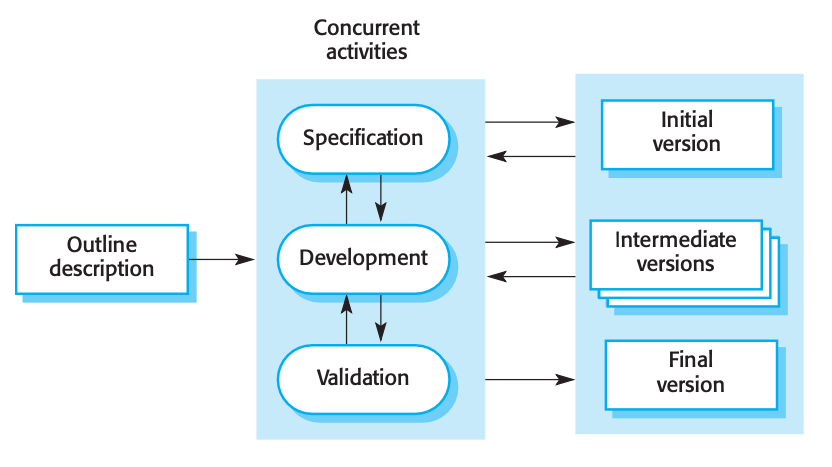
\includegraphics[scale=0.3]{img/incrementale.png}
\end{figure}
\subsubsection{Vantaggi e svantaggi}

Il modello di sviluppo incrementale offre il vantaggio di ridurre i costi
nel rispondere ai cambiamenti dei requisiti del cliente. A differenza del
modello a cascata, richiede meno analisi e documentazione da rifare, facilitando
l'ottenimento del feedback del cliente sul lavoro di sviluppo compiuto fino a quel
momento. I clienti possono commentare le dimostrazioni e monitorare i progressi,
consentendo la consegna e l'implementazione rapida delle parti più utili del software.
In questo modo, i clienti sono in grado di utilizzare il software, seppur parziale,
più precocemente rispetto a un processo a cascata.

Questo approccio stimola inoltre il cambiamento, che di fatto potrebbero non 
emergere non vedendo il sistema in esecuzione. Il committente che non ha chiaro 
il requisito da sviluppare, vedendo il sistema all'opera riesce a ragionare concretamente
e quindi stimola delle riflessioni che astrattamente non venivano espresse.

Le incomprensioni, inoltre, emergono fin da subito, permettendo di risolvere i problemi 
in maniera tempestiva.

Avere a disposizioni versioni precoci del sistema permette, oltre che ad avere feedback,
anche il trasferimento di valore al cliente, permettendo a delle funzionalità di essere 
già utilizzate nel business.

Tuttavia, il processo presenta anche delle sfide. 
Il processo non è monitorabile come nel processo guidato da piani, perché di fatto 
non ci sono obiettivi che vengono raggiunti o un documento dei 
requisiti che viene consegnato ad un certo punto e quindi, specialmente per il 
management è difficile avere una chiara visione dell'andamento dello sviluppo, capendo 
se si è in linea con le scadenze, o comunque non è così esplicito come con 
l'ausilio di waterfall.
Questo è uno dei motivi per la quale questo tipo di processo ha un po' di resistenze, soprattutto 
in progetti costosi di grandi dimensioni.
Inoltre, la documentazione è molto minimale e potrebbe essere obsoleta rispetto 
alla versione corrente del software. Potrebbe essere che l'architettura ideata inizialmente 
potrebbe non essere adatta a recepire, trovandoci quindi ad dover scendere a compromessi,
riadattando funzionalità, causando la degradazione del sistema, richiedendo quindi 
che si spenda del tempo nell'attività di \textbf{refactoring}. Non dare la giusta importanza 
a tale attività può portare alla corruzione della struttura.

\subsection{Integrazione e configurazione}
Nel processo di sviluppo software di integrazione e configurazione, 
invece di puntare sullo sviluppo del codice sorgente da zero, si punta ad integrare 
componenti che si trovano sullo \textit{scaffale}, integrando quindi pezzi pronti
per le singole funzionalità richieste, e il maggior sforzo sarà relativo alla 
configurazione, ovvero la scrittura di codice \textit{colla} che cerca di mettere
insieme queste componenti per realizzare le funzionalità richieste.

Lo sviluppo di software basato sul riutilizzo è un approccio in cui i sistemi
sono integrati a partire da componenti o sistemi già esistenti. Questo metodo
sfrutta in particolare i componenti Commercial-off-the-shelf (\texttt{COTS}),
che sono sistemi disponibili commercialmente o all'interno dell'azienda
e possono essere riutilizzati così
come sono o configurati per adattarsi alle esigenze e ai requisiti specifici degli
utenti. Gli elementi riutilizzati possono essere configurati per adattare il loro
comportamento e le loro funzionalità, rendendo il riutilizzo l'approccio standard
per la costruzione di molti tipi di sistemi aziendali.

Lo sforzo è mirato verso la \textbf{selezione dei componenti giusti} e all'integrazione 
di questi nel sistema finale.
Si parla di configurazione perché spesso si tratta di componenti \textit{general purpose},
e più che implementazione lo sforzo è relativo alla configurazione dei parametri operativi,
in modo che siano efficaci nel sistema che si va a sviluppare.

\begin{figure}[H]
    \centering
    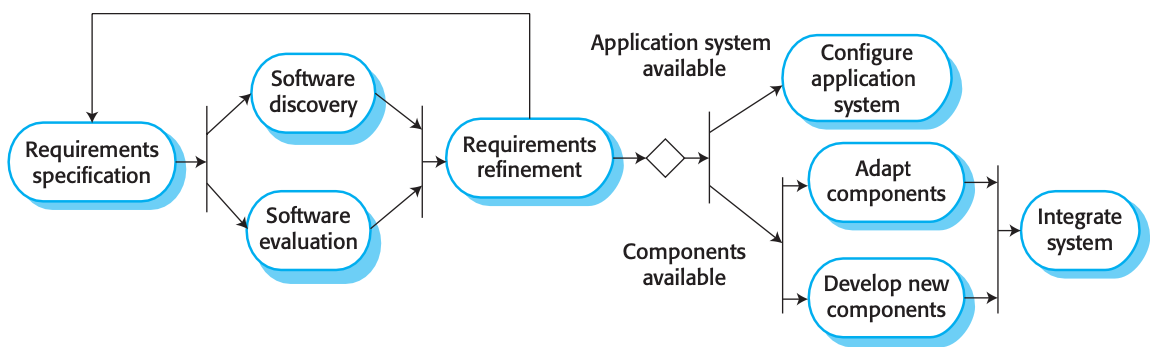
\includegraphics[scale=0.35]{img/integr_config.png}
\end{figure}

\subsubsection{Commonly used components - \texttt{COTS}}
I sistemi autonomi (\texttt{COTS}), generalmente dotati di numerose funzionalità, vengono
adattati o configurati per l'uso in un ambiente specifico. Si trovano anche collezioni
di oggetti sviluppati come pacchetti da integrare con un framework di componenti,
come ad esempio \texttt{Java Spring}. In aggiunta, vi sono i servizi web sviluppati secondo
gli standard di servizio e che sono disponibili per l'invocazione remota. Questa
pluralità di opzioni disponibili per il riutilizzo nel software fornisce una
flessibilità senza precedenti nella progettazione e nello sviluppo di nuovi sistemi,
consentendo alle aziende di risparmiare tempo e risorse.
\subsubsection{Specifica dei requisiti}
Nella fase iniziale si individuano le funzionalità che il sistema dovrà mettere a disposizione
ad alto livello. Tipicamente si tratta di una descrizione essenziale che il sistema dovrà avere,
perché i requisiti dovranno piegarsi a quelle che sono le funzionalità disponibili dalle 
componenti già pronte per essere integrate.
\subsubsection{Fase di ricerca e valutazione dei componenti}
Le fasi di ricerca e valutazione dei componenti si svolgono in parallelo.
Nella fase di ricerca si cercano nelle componenti le funzionalità che 
sono state identificate, mentre nella fase di valutazione, nel caso in cui più componenti 
espongano la stessa funzionalità, si decide quale utilizzare si in termini di \textbf{integrabilità}
che in termini di \textbf{funzionabilità}.
\subsubsection{Affinamento dei Requisiti}
A questo punto di procede con l'affinamento dei requisiti, cercando di comprendere se 
le componenti soddisfano appieno i requisiti prefissati e si valuta se accettare 
requisiti leggermente diversi in modo da utilizzare le componenti a disposizione, 
e in questo caso di itera in questo ciclo finché di raggiunge un allineamento tra le componenti 
disponibili e i requisiti prefissati.
\subsubsection{Configurazione del sistema}
Se di fatto i componenti individuati forniscono una copertura completa dei requisiti possiamo 
iniziare a \textbf{configurare} tali componenti, rendendo il sistema finale di fatto 
composto dalle componenti selezionate. 
\subsection{Adattamento delle componenti e sviluppo delle componenti}
Nel caso in cui il sistema non risulta configurabile, dobbiamo o adattare le componenti 
disponibili o sviluppare nuove componenti, per poter \textbf{integrare il sistema}. 
\subsection{Vantaggi e svantaggi}
I vantaggi sono legati al basso costo, al rischio basso, dato che le componenti sono 
già state testate e sviluppate in precedenza (\textit{sia da terzi che da progetti esistenti}).
Il software da sviluppare è poco, rendendo di fatto il team di sviluppo abbastanza piccolo e 
il sistema viene consegnato in tempi brevi. Questo approccio è tipicamente adottato in caso di 
startup, dove c'è la necessità di raggiungere il mercato il più presto possibile, potendo quindi 
trasferire valore dal mercato all'azienda.

Gli svantaggi sono legati alla qualità del prodotto più bassa, nel senso che spesso è 
necessario adottare dei compromessi e quindi avere soluzioni non pienamente ottimali.
Come effetto collaterale della qualità bassa, il sistema finale potrebbe non rispondere 
ai requisiti completi dei miei utenti.
Lo svantaggio principale è dovuto al fatto che non c'è controllo dell'evoluzione del 
sistema software, poiché lo sviluppo dei singoli componenti è in capo alla azienda o 
comunità che ha sviluppato quel componente, quindi se dovessero esserci dei problemi 
legati all'implementazione dei componenti, io come team di sviluppo, non ho pieno
controllo sui tempi necessari per risolvere tale problema.

\section{Attività di sviluppo software}
Le attività comuni che il processo di sviluppo software deve affrontare sono:
\begin{itemize}
  \item \textbf{Specifica}: definizione dei requisiti del sistema;
  \item \textbf{Design e Implementazione}: definizione dell'organizzazione del sistema e
  la sua realizzazione;
  \item \textbf{Validazione}: verifica che il sistema sia conforme alle specifiche;
  \item \textbf{Evoluzione}: modifica del sistema in risposta al cambiamento 
  dei bisogni degli utenti.
\end{itemize}
\subsection{Specifica}
La specifica delle funzionalità, nota anche come \textbf{ingegneria dei requisiti},
è il processo che mira a capire e a definire quali servizi sono richiesti e identificati 
per lo sviluppo del sistema. 
Questo processo è uno dei processi più critici del ciclo di vita del software, poiché
un errore in questa fase comporterà sicuramente dei problemi nel sistema finale, potendone 
causare il fallimento. 

Talvolta, è opportuno condurre un'attività preliminare di \textbf{studio di fattibilità}
per verificare se il sistema proposto è fattibile dal punto di vista tecnico, economico
e organizzativo. Di fatto si tratta di una versione in miniatura del progetto che 
permette di valutare se avviare o meno il progetto.

Tipicamente questa fare produce un \textbf{documento dei requisiti} che definisce
formalmente i requisiti del sistema. Questo documento deve essere comprensibile sia
per i clienti che per gli sviluppatori.
\subsubsection{Produrre un documento dei requisiti}
\begin{enumerate}
    \item \textbf{Elicitazione dei requisiti}: per elicitazione, di fatto, si vuole intendere 
    l'attività di trasferimento delle funzionalità richieste dal cliente 
    verso gli ingegneri dei requisiti e/o del software. Consiste quindi in una descrizione 
    del sistema che può essere fatta in vari modi (\textit{interviste, questionari, osservazione 
    di sistemi software precedenti, studio di documentazione, ecc...}). Tale fase potrebbe 
    richiedere anche la realizzazione di prototipi per aiutare il cliente a capire meglio
    le sue esigenze.
    \item \textbf{Specifica dei requisiti}: i requisiti, una volta raccolti, devono essere
    specificati, ovvero devono essere descritti in modo preciso e non ambiguo. La rappresentazione
    dei requisiti può essere fatta in vari modi (\textit{scrittura di documenti,
    modelli grafici, modelli matematici, ecc...}), l'importante è che possa permettere
    il dialogo tra i clienti e gli sviluppatori.
    
    I requisiti possono essere classificati in due categorie:
    \begin{itemize}
        \item \textbf{User Requirements}: descrivono le funzionalità del sistema dal punto
        di vista degli utenti, che sono interessanti per il cliente, poiché descrivono
        ciò che il cliente vuole dal sistema;
        \item \textbf{System Requirements}: descrivono le funzionalità del sistema dal punto
        di vista degli sviluppatori, che sono interessanti per gli sviluppatori, poiché 
        descrivono ciò che il sistema deve fare.
    \end{itemize}
    \item \textbf{Validazione dei requisiti}: Una volta che i requisiti sono stati
    specificati, è necessario verificarli per assicurarsi che siano corretti, completi
    e realistici, 
    catturando quindi tutte le funzionalità richieste dal cliente e che non ci siano
    ambiguità. L'attività prevede che vi sia anche un controllo di errori e omissioni.
    In caso di errori il documento dei requisiti deve essere corretto e aggiornato.
\end{enumerate}
\begin{figure}[H]
  \centering
  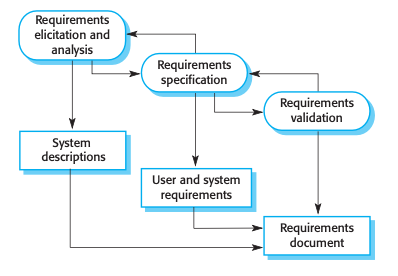
\includegraphics[scale=0.5]{img/requisitifasi.png}
  \caption{Processo di produzione di un documento dei requisiti}
\end{figure}
Ognuna di queste fasi può opzionalmente avere un \textit{deliverable}, ovvero un
documento che viene prodotto e utilizzo come input per la fase successiva.
A seconda dell'approccio di sviluppo ci saranno step più o meno formali.
\subsection{Design e implementazione}
Questa fase consiste nel definire l'architettura del sistema e di fatto implementarlo
mediante la scrittura del codice sorgente che rappresenta l'implementazione del sistema.

Per \textbf{design} si intende la definizione delle \textit{strutture dati} che dovranno essere 
implementare, i \textit{modelli} e le strutture utilizzate dal sistema, le \textit{interfacce} 
che verranno utilizzate per comunicare con il sistema, gli \textit{algoritmi} che verranno utilizzati
per implementare le funzionalità del sistema e le \textit{procedure di comunicazione} tra le varie
componenti del sistema.

L'\textbf{implementazione} consiste nella scrittura del codice eseguibile che implementa
le funzionalità del sistema.

Tipicamente il design del sistema è organizzato in quattro attività:
\begin{enumerate}
    \item \textbf{Design architetturale}: ad alto livello si individuano le macro 
    aree in cui il sistema verrà articolato. Definendo quindi i principali componenti
    del sistema e le loro interazioni. 
    \item \textbf{Design del database}: si definiscono le strutture dati utilizzate 
    ad alto livello e come 
    verranno rappresentate nel database.
    \item \textbf{Design dell'interfacce}: si definiscono le interfacce che verranno
    utilizzate per comunicare con il sistema, poiché è importante definire come verranno
    scambiate le informazioni tra il sistema e l'ambiente esterno. Nel concreto, è importante 
    definire l'interfaccia perché permette gli sviluppatori di essere guidati nella scrittura
    del codice.
    \item \textbf{Selezione e design dei componenti}: una volta definite le interfacce
    e le loro funzionalità è possibile 
    procedere per la ricerca di componenti disponibili sul mercato che soddisfano 
    le caratteristiche di cui si ha bisogno.
    Nel caso in cui non si trovino componenti adatti, è necessario progettare i componenti
    che verranno utilizzati. 
    I componenti non riutilizzabili vengono progettati e implementati.
\end{enumerate}
La progettazione ha una struttura gerarchica, ovvero si parte da un livello più alto
e si scende di livello fino ad arrivare al livello più basso. Questo è importante 
soprattutto per progetti software di grandi dimensioni, poiché permette di suddividere
il lavoro in modo più semplice e di gestire meglio le risorse.
\subsection{Verifica e validazione}
Una volta che il sistema è stato implementato e anche durante lo sviluppo 
del software, è necessario verificare che il sistema
sia allineato ai requisiti fissati. 
Per farlo è possibile utilizzare due approcci:
\begin{itemize}
    \item \textbf{Verifica}: consiste nell'ispezionare il codice sorgente, ragionando 
    sul codice scritto, per capire se il codice è corretto e se soddisfa i requisiti.
    \item \textbf{Testing}: consiste nell'eseguire il codice sorgente, per capire se
    il comportamento osservato è corretto e se soddisfa i requisiti (\textit{anche 
    mediante dati simulati}).
\end{itemize}

Anche il testing si divide in sotto-fasi:
\begin{enumerate}
    \item \textbf{Testing del componente}: si testa il componente singolarmente,
    per capire se il componente se la responsabilità del componente è corretta.
    \item \textbf{Testing di integrazione}: si testa l'integrazione tra le varie componenti.
    \item \textbf{Testing del sistema}: si testa il sistema nel suo complesso,
    per capire se il sistema funziona correttamente. Si verifica che l'integrazione 
    tra i vari componenti sia corretta.
    \item \textbf{Accettazione del testing \textit{customer testing}}: si testa il sistema
    in un ambiente simile a quello in cui verrà utilizzato, anche con 
    dati realistici, per capire se il sistema
    soddisfa i requisiti fissati.
\end{enumerate}
\subsubsection{Modello a V}
Quando si adotta questa tipologia di test gerarchico, si parla di modello a V della 
verifica e validazione.
\begin{figure}[H]
    \centering
    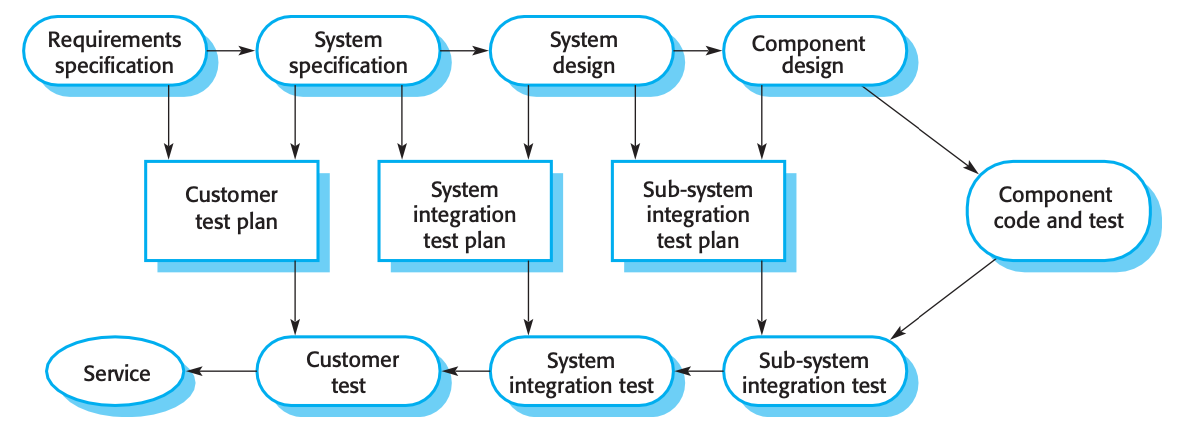
\includegraphics[scale=0.3]{img/validation.png}
    \caption{Modello a V della verifica e validazione}
\end{figure}
Il piano di test viene elaborato in modo inverso rispetto al piano di sviluppo.
Inizialmente, quando le funzionalità che il sistema deve offrire vengono stabilite,
si definiscono i test di accettazione, che saranno gli ultimi a essere eseguiti,
solo dopo che il sistema è stato completamente implementato. Successivamente, una
volta che l'architettura del sistema è stata delineata, si procede con la definizione
del piano di test a livello di sistema. Man mano che i singoli componenti vengono
specificati, si definiscono anche i test per ciascuno di questi componenti. In
questo modo, i test sono pianificati partendo dal livello più alto fino a quello
più basso,
ma la loro esecuzione avviene in ordine inverso, dal più basso al più alto.
\subsection{Evoluzione del software}
\begin{figure}[H]
    \centering
    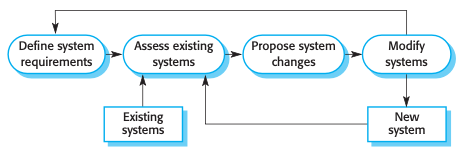
\includegraphics[scale=0.7]{img/evolution.png}
    \caption{Processo di evoluzione del software}
\end{figure}
Quando si ritiene necessario apportare una modifica, può essere seguito uno schema
di evoluzione del software, che prevede le seguenti fasi:
\begin{enumerate}
    \item \textbf{Definizione dei requisiti di sistema}: si definisce il cambiamento che si vuole
    apportare al sistema, ovvero si definisce il requisito che si vuole aggiungere o
    modificare.
    \item \textbf{Analisi dell'impatto}: si analizza l'impatto che il cambiamento avrà
    sul sistema, ovvero si analizza quali componenti del sistema verranno modificati
    e quali no. Per impatto si intende anche il costo che il cambiamento avrà sul sistema,
    e come tale dovrà essere negoziato con il cliente.
    \item \textbf{Progettazione del cambiamento}: si ritorna dal cliente per unificare 
    se il cambiamento è accettabile e se il costo è accettabile. 
    \item \textbf{Implementazione del cambiamento}: si implementa il cambiamento.
\end{enumerate}

\section{Gestione dei cambiamenti}
Nel contesto del processo di sviluppo del software, è essenziale gestire efficacemente
i cambiamenti per garantire una transizione fluida e un prodotto finale di alta qualità.
Tre aspetti chiave della gestione dei cambiamenti sono:

\begin{enumerate}
    \item \textbf{Cambiamenti che causano rilavoro e introduzione di nuove funzionalità:}
    Durante lo sviluppo, possono emergere richieste di modifiche o l'aggiunta di nuove
    funzionalità. È importante essere pronti ad affrontare queste modifiche,
    ma bisogna anche considerare l'impatto sul lavoro già svolto.
    
    \item \textbf{Anticipazione dei cambiamenti:} Un approccio preventivo consiste
    nell'anticipare possibili modifiche prima che diventino necessari
    rilavori significativi. Ad esempio, condividere un prototipo con gli utenti finali
    per discutere e finalizzare i loro requisiti prima di impegnare notevoli risorse
    nell'implementazione definitiva.
    
    \item \textbf{Tolleranza ai cambiamenti:} Il processo di sviluppo dovrebbe essere
    progettato in modo da consentire l'incorporazione di cambiamenti a un costo
    relativamente basso. Questo significa che le modifiche non dovrebbero comportare
    una revisione completa del lavoro svolto fino a quel momento.
\end{enumerate}
\subsection{Prototipazione}
È anche importante menzionare il ruolo del prototipo nell'ambito dello
sviluppo del software:
\begin{tcolorbox}[title = Prototipo]
    Il prototipo aiuta a rendere tangibile un concetto che altrimenti
    sarebbe astratto. Permette di esplorare diversi approcci per implementare
    un cambiamento, come modifiche all'architettura o all'interfaccia utente,
    senza apportare modifiche dirette al sistema. Questo processo facilita il
    team di sviluppo nella comprensione di come minimizzare l'impatto dei
    cambiamenti. Inoltre, consente una convalida efficace
    del cambiamento con il cliente.
\end{tcolorbox}
Lo sviluppo rapido e iterativo del prototipo aiuta a controllare i costi.
Durante l'ingegneria dei requisiti, il prototipo aiuta la fase di elicitazione
dei requisiti e
nella validazione dei requisiti del sistema, per capire se un requisito è stato appreso
correttamente, o per aiutare i clienti ad esprimere idee che altrimenti risulterebbero 
astratte. Durante la progettazione del
sistema, può essere utilizzato per esplorare soluzioni nell'ambito dell'interfaccia
utente.
\subsection{Gestione del cambiamento nell'Approccio Incrementale}
Quando abbiamo riportato il processo di sviluppo incrementale, avviamo detto che 
si tratta del processo di sviluppo che si presta meglio alla gestione dei cambiamenti
perché prevede diverse consegne al cliente e quindi il cambiamento avviene proprio 
per natura del processo. I cambiamenti possono essere legati ai requisiti, ma anche
a nuove funzionalità che il cliente vuole aggiungere, di natura tecnica legata
all'implementazione o esigenze di mercato.

Il cliente può sperimentare il sistema, fornire feedback e richiedere modifiche
prima che il prodotto sia completato. Questo approccio consente di ridurre il rischio
di fallimento del progetto e di garantire che il prodotto soddisfi le esigenze del
cliente. 

Il prodotto in questo modo sarà facilmente allineato con le necessità del cliente,
che potevano non essere chiare all'inizio del progetto, non avendo avuto modo di
integrare il sistema software con il proprio ambiente di lavoro.
\subsection{Vantaggi e svantaggi dell'approccio incrementale}
Le funzionalità del sistema sono disponibili in tempi brevi, il che consente
di ottenere un feedback rapido dal cliente. Questo feedback può essere utilizzato
per guidare lo sviluppo futuro e garantire che il prodotto soddisfi le esigenze
del cliente. Inoltre, le consegne incrementali sono funzionali per la fase 
di elicitazione dei requisiti, in quanto consentono di esplorare i requisiti
con il cliente e di ottenere un feedback immediato.
Si ha minor rischio di fallimento del progetto, in quanto il prodotto viene
consegnato in piccole parti, e quindi è più facile correggere eventuali errori
e allinearsi con le esigenze del cliente, dando inoltre priorità alle funzionalità
più importanti che saranno quelle maggiormente testate e quindi più affidabili.

Gli svantaggi sono legati al fatto che la maggior parte dei progetti software,
anche per le prime versioni, richiedono un \textbf{grosso sottoinsieme} di funzionalità
per essere utilizzabili, non permettendo quindi di trasferire immediatamente 
valore al cliente, che è il principale obiettivo del processo incrementale.
Inoltre, la specifica delle funzionalità viene sviluppata insieme al sistema,
non avendo quindi modo di congelare un documento dei requisiti per verificare 
in maniera rigorosa e completa i requisiti del sistema.
Non è possibile quindi applicare tale approccio in commesse governative o 
ministeriali in cui i requisiti sono ben definiti nel contratto
e non possono essere modificati
durante il processo di sviluppo.